%%%%%%%%%%%%%%%%%%%%%%%%%%%%%%%%%%%%%%%%%
% a0poster Portrait Poster
% LaTeX Template
% Version 1.0 (22/06/13)
%
% The a0poster class was created by:
% Gerlinde Kettl and Matthias Weiser (tex@kettl.de)
% 
% This template has been downloaded from:
% http://www.LaTeXTemplates.com
%
% License:
% CC BY-NC-SA 3.0 (http://creativecommons.org/licenses/by-nc-sa/3.0/)
%
%%%%%%%%%%%%%%%%%%%%%%%%%%%%%%%%%%%%%%%%%

%----------------------------------------------------------------------------------------
%	PACKAGES AND OTHER DOCUMENT CONFIGURATIONS
%----------------------------------------------------------------------------------------

\documentclass[a0,portrait]{a0poster}

\usepackage{multicol} % This is so we can have multiple columns of text side-by-side
\columnsep=100pt % This is the amount of white space between the columns in the poster
\columnseprule=3pt % This is the thickness of the black line between the columns in the poster

\usepackage[svgnames]{xcolor} % Specify colors by their 'svgnames', for a full list of all colors available see here: http://www.latextemplates.com/svgnames-colors

\usepackage{times} % Use the times font
%\usepackage{palatino} % Uncomment to use the Palatino font

\usepackage{graphicx} % Required for including images
\graphicspath{{figures/}} % Location of the graphics files
\usepackage{booktabs} % Top and bottom rules for table
\usepackage[font=small,labelfont=bf]{caption} % Required for specifying captions to tables and figures
\usepackage{amsfonts, amsmath, amsthm, amssymb} % For math fonts, symbols and environments
\usepackage{wrapfig} % Allows wrapping text around tables and figures


\usepackage[shortlabels]{enumitem}
\begin{document}

%----------------------------------------------------------------------------------------
%	POSTER HEADER 
%----------------------------------------------------------------------------------------

% The header is divided into two boxes:
% The first is 75% wide and houses the title, subtitle, names, university/organization and contact information
% The second is 25% wide and houses a logo for your university/organization or a photo of you
% The widths of these boxes can be easily edited to accommodate your content as you see fit

\begin{minipage}[H]{0.7\linewidth}
\veryHuge \color{NavyBlue} \textbf{Ranking Official Websites of UMJI} \color{Black}\\ % Title
\Huge\textit{Using PageRank and Markov Chain}\\[2cm] % Subtitle
\huge \textbf{Author: Yi SUN \& Tianbo CHEN \& Zhuoer ZHU}\\
\huge \textbf{Instructor: Olga Danilkina}\\[0.5cm] % Author(s)
\Large UNIVERSITY OF MICHIGAN - SHANGHAI JIAO TONG UNIVERSITY JOINT INSTITUTE\\[0.4cm] % University/organization
\end{minipage}
%
\begin{minipage}[l]{0.3\linewidth}

\includegraphics[width=\linewidth]{JI_logo}\\
\end{minipage}

\vspace{1cm} % A bit of extra whitespace between the header and poster content

%----------------------------------------------------------------------------------------

\begin{multicols}{2} % This is how many columns your poster will be broken into, a portrait poster is generally split into 2 columns

%----------------------------------------------------------------------------------------
%	ABSTRACT
%----------------------------------------------------------------------------------------




%----------------------------------------------------------------------------------------
%	INTRODUCTION
%----------------------------------------------------------------------------------------


\color{Navy} 
\section*{Introduction}
 \paragraph{}
    It's common for a freshman to suffer from the transition period from his high school to the university. In order to get accustomed to the new environment one might well visit the official websites of his university and gather as much information as he can. However, the official website may include tons of links among which many are useless and out of date.
 
    Therefore, to help freshman of the Joint Institute get familiar with online campus life, we are going to rank the importance of umji official websites (umji.sjtu.edu.cn) using what we learned in VV214 Linear Algebra. Meanwhile, this method can also be used for other departments and universities.

%----------------------------------------------------------------------------------------
%	OBJECTIVES
%----------------------------------------------------------------------------------------
\color{SaddleBrown} % SaddleBrown color for the introduction


\section*{Previous Studies}

\paragraph{}
    First developed by Larry Page and Sergey Brin in 1996, PageRank Algorithm is an eigenvalue problem[1]. 
    Web pages are ranked according to the fundamental assumption that a page is more important if it is pointed to by more pages.
    
    The algorithm soon brought him an idea of a large-scale hypertextual web search engine[2], which is later named as Google.
    They introduced the natural model of PageRank Algorithm, including the damping factor $\alpha$. 
    To be exact, $\alpha$ is the probability that, at any step, a random surfer would continue his trip from page i to page j.
    The residual probability is estimated from the frequency that an average surfer uses the bookmark feature in his browser. It is generally assumed that $\alpha\approx0.85$.
    
    The Google search engine was proved to be relatively efficient, for sake of the large eigengap of its transition matrix[3]. 
    As a result, the stationary probability of a random visitor arriving at page i could be approximated through a few iteration of the power method.

%----------------------------------------------------------------------------------------
%	MATERIALS AND METHODS
%----------------------------------------------------------------------------------------



\color{DarkSlateGray} % DarkSlateGray color for the rest of the content
%------------------------------------------------

\section*{Mathematical Background}
\subsection*{Eigenvalue $\&$ Eigenvector}
        \paragraph{}
        Let M be an $n\times n$ matrix. In linear algebra, we denotes that: 
            1) if $x^TM=\lambda x^T$, x is called a left eigenvector.
            2) if $Mx=\lambda x$, x is called a right eigenvector.
            3) a left eigenvector is the corresponding right eigenvector of $M^T$.
        
      \subsection*{Markov Chain}
      \subsubsection*{Discrete Time Markov Chain}
        \paragraph{}
        In statistics and probabilities, Markov property denotes the momeoryless property of a stochastic / random process, i.e.,
        $P[X_{n+1=x_{n+1}}\vert X_n=x_n,\cdots X_0=x_0]=P[X_{n+1=x_{n+1}}\vert X_n=x_n]$
        
        \paragraph{}
        A Discrete Time Markov Chain is a sequence of state spaces $S={P[X_i]}$ connected by directed edges, and satisfies the Markov property.
        The n-th edge of the state space is a transition probability matrix, with $p_{ij}=P[X_i->X_j]$.
        By definition, the transition matrix satisfies $\sum_{i=1}^{dim S}$ [$p_{ai}$] = 1, $\forall a$.
      \subsection*{Natural PageRank Model}
      \paragraph{}
        The PageRank Algorithm ranks the importance of web pages. It is assumed that, the more outbound links a page receives, the more important the page is.
        \subsubsection*{Ideal PageRank Model}
        \paragraph{}
        Ideal PageRank Model views the web as a directed graph G=(V,E), where each of the N pages $\in V$ is a node, and each hyperlink $\in E$ is an edge.
        The adjacency matrix A of the graph stores the out-degree of vertex i. If $\sum^n_{j=1}a_{ij}=0$, the corresponding page i is a dangling node with no out-links.
        
        We construct a Markov Chain with a state space S=V for page 1 to N. Row-stachastic vector $x_n=\left[P_{page1}\;P_{page2}\;\cdots\;P_{pageN}\right]^T$.
        A random surfer is supposed to pick a page $\in V$ at the probabilities discribed by 
        transition matrix P, where $p_{ij}=\frac{1}{outdeg(i)}$ for every page j adjacent to i.
        
        Given P and Perron-Frobenius Theorem, stationary distribution $\overline{x_\infty}$ could be obtained from 
        : 1) $x^T=x^TP$.
          2) $\overline{x_\infty}$=$\frac{x}{||x||}$.
      
        \subsubsection*{Dangling Nodes}
        \paragraph{}
        At the presence of dangling nodes, the random surfer cannot go to any other pages since there is no outbound links on the page, namely, $\sum^n_{j=i}p_{ij}=0$. 
        The iteration of Markov Chain is stucked in the ideal model.
        
        We solve this problem by introducing a new transition matrix $\overline{P}$=P+D, where D=$\textbf{dv}^T$, $d_i=1$ iff outdeg(i)=0, and $\textbf{v}$ is a general surfer preference for pages $\in$ V.
        \subsubsection*{Cyclic Paths}
        \paragraph{}
        Similarly, the surfer might get trapped by a cyclic path in G. $\overline{x_n}$ would never converge to $\overline{x_\infty}$ under this circumstance.
        
        It is artificially defined to avoid this reducibility that, at every time t, the surfer would continue to click the outbound links with a high probability $\alpha\approx0.85$, while jump to all nodes with the probability $(1-\alpha)\cdot100\%$.
        
        The ultimate transition matrix for the natural PageRank Model is thus
        $\hat{P}=\alpha\overline{P}+(1-\alpha)\textbf{ev}^T$,
        where $\textbf{e}$ is a row vector with all entries equal to 1.
        \subsubsection*{Eigenproblem}
        \paragraph{}
        Up to now, the PageRank problem is simplified as a eigenproblem $\textbf{z}^T\hat{P}=\textbf{z}^T$, where $\textbf{z}$ is the PageRank vector we are looking for.
        
        A common method to solve this eigenproblem is the power method. Previous studies have concluded that for the rank-one modification of $\alpha P$, $\hat{P}$, few steps of iteration in power method would be enough for a relatively precise $\textbf{z}$.
        
        Note that $\textbf{z}^T\textbf{e}=\sum^N_{i=1}z_i=1$,
        this eigenproblem can be rewritten into a linear system
        $S\textbf{z}=(1-\alpha)\textbf{v}$,
        where S=I-$\alpha P^T-\alpha\textbf{vd}^T$.
        
        We would further discuss the handling of the nonsparsity of S so as to reduce the complexity of PageRank Algorithm.
\subsection*{Fast PageRank via Sparse Linear system}
\paragraph{}
To handle the problem in a more efficient way, we can take the advantage of the sparse linear system which is common in real life dealing with web searching PageRank problems.  According to Kamvar et al. [4], a 2001 sample of the web containing 290 million pages had only 70 million nondangling nodes. Therefore, the matrix $P$ is quite sparse.
\subsubsection*{Sparse Matrix}
\paragraph{}
A matrix is defined to be sparse if its sparsity is greater than 0.5, where the sparsity is the number of zero-valued elements divided by the total number of elements. From Douglas[5], when dealing with a  linear system involves a sparse matrix, we can find a reordering scheme that can increase data locality and decrease the computation time . For example, a very effective reordering scheme, denoted by $B$, is the one obtained by permuting the nodes of the web graph according to the order induced by a BFS visit.

\subsubsection*{How to Exploit Sparse Matrix}
\paragraph{}
From Del Corso et al. Theorem 4.2[6], we can convert the problem to a equivalent one: solving $R\mathbf{y}=\mathbf{v}$, where $R=I-\alpha P^T$. Then, we can get $\mathbf{z} = \mathbf{y}/ ||\mathbf{y}||_1$. Since $I$ and $P$ are sparse matrix, we can easily identify $R$ as a sparse matrix. Therefore, we can use the property of sparse linear system to solve the PageRank problem in a more efficient way.

\color{purple}
\section*{Problem}
\paragraph{}
   We choose 40 websites which linked to the homepage of \textbf{UMJI}, \textit{http://umji.sjtu.edu.cn/} to investigate into.
   \subsection*{Power iteration}
   \paragraph{}
   A common method to solve then eigenproblem $z^{T}\hat{P} = z^T$ is \textit{power iteration}\\
  \begin{minipage}[H]{1\linewidth}
  	\centering
  	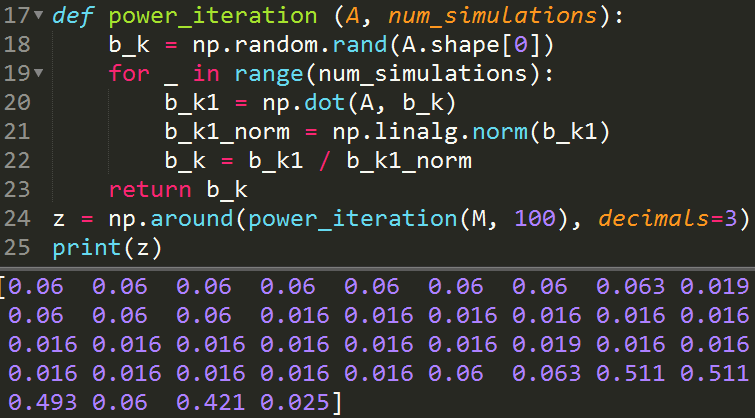
\includegraphics{result.PNG}
  	\label{Table 1}
  \end{minipage}
   \subsection*{Faster PageRank}
   \paragraph{}
   Find all \textit{strong connected components} by \textit{BFS} algorithm to split the original linear system $Ry=v$ into smaller linear systems, which reduced the size of our problem. Then apply \textit{power method} to solve each linear systems and combine the solutions together.
  \subsection*{Result}
  \paragraph{}
  According to the result of our program, four most important pages are \textit{http://umjicanvas.com}, \textit{http://en.sjtu.edu.cn}, \textit{http://www.umji.sjtu.edu.cn} and \textit{http://weibo.com/umsjtuji}.   

\color{teal}
\section*{Conclusions}
  \paragraph{}
  The main idea of Fast PageRank Computation via a Sparse Linear System is based on the thought of divide and conquer, and our eigenproblem can be solved easily because of the properties of stochastic sparse matrix. However, power iteration is simple, inefficient and non-universal. Nowaday many methods like \textit{Arnoldi iteration} are used for different kind of eigenproblems, such as the problem of users recommendations for social network service websites like Facebook and twitter.

\color{DarkSlateGray} % Set the color back to DarkSlateGray for the rest of the content

%----------------------------------------------------------------------------------------
%	FORTHCOMING RESEARCH
%----------------------------------------------------------------------------------------


 %----------------------------------------------------------------------------------------
%	REFERENCES
%----------------------------------------------------------------------------------------

\nocite{*} % Print all references regardless of whether they were cited in the poster or not
\bibliographystyle{plain} % Plain referencing style
\bibliography{sample} % Use the example bibliography file sample.bib

%----------------------------------------------------------------------------------------
%	ACKNOWLEDGEMENTS
%----------------------------------------------------------------------------------------

\section*{Reference}
\begin{enumerate}
\item[[1]] Page, Larry, "PageRank: Bringing Order to the Web". 
Archived from the original on May 6, 2002. Retrieved 2016-09-11., 
Stanford Digital Library Project, talk. August 18, 1997 

\item[[2]] Brin, S.; Page, L. (1998). "The anatomy of a large-scale hypertextual Web search engine". 
Computer Networks and ISDN Systems. 30 (1–7): 107–117. CiteSeerX 10.1.1.115.5930. doi:10.1016/S0169-7552(98)00110-X. ISSN 0169-7552. 

\item[[3]] Taher Haveliwala; Sepandar Kamvar (March 2003). "The Second Eigenvalue of the Google Matrix". 
Stanford University Technical Report: 7056. arXiv:math/0307056. Bibcode:2003math......7056N. 

\item[[4]] S. D. Kamvar, T. H. Haveliwala, C. Manning, and G. H. Golub. “Exploiting the Block Structure of the Web for Computing PageRank.” Technical report, Stanford University, 2003.

\item[[5]] C. Douglas, J. Hu, M. Iskandarani, M. Kowarschik, U. R¨ude, and C. Weiss. “Maximizing Cache Memory Usage for Multigrid Algorithms.” In Multiphase Flows and Transport in Porous Media: State of the Art, edited by Z. Chen et al., pp. 124–137. 

\item[[6]] Gianna M. Del Corso, Antonio Gulli, and Francesco Romani. "Fast PageRank Computation via a Sparse Linear System." Internet Mathematics Vol. 2, No. 3: 251- 273, 2005.
\end{enumerate}

%----------------------------------------------------------------------------------------

\end{multicols}
\end{document}